\documentclass{article}
\usepackage{textcomp,mathrsfs}
\usepackage{graphicx,amssymb,amsmath,amsthm,mathrsfs}
\usepackage{multirow,makeidx,algorithmic,algorithm}
\usepackage{latexsym,graphicx,amssymb,amsmath,amsthm,mathrsfs}
\usepackage{mathrsfs}
\usepackage{amssymb}
\usepackage{booktabs,fancyhdr} 
\usepackage{rotating}
\usepackage{pdflscape}
\usepackage{array}
\usepackage{stmaryrd}
\usepackage{enumerate}
%\usepackage[authoryear,comma,longnamesfirst,sectionbib]{natbib}
\usepackage[numbers]{natbib}
\usepackage{color}

\usepackage[left=2.54cm,top=2cm,right=2cm,bottom=2.54cm]{geometry}


% \usepackage[usenames,dvipsnames]{color}
% \usepackage[frenchb]{babel}



% This gives you control over how far down in the hierarchy the
% table of contents will print.
\setcounter{tocdepth}{3}
\setcounter{secnumdepth}{3}

 
\usepackage{url}
%%%%% URL package fix %%%%%
\begingroup
\makeatletter
\g@addto@macro{\UrlSpecials}{%
  \endlinechar=13 \catcode\endlinechar=12
  \do\%{\Url@percent}\do\^^M{\break}}
 \catcode13=12 %
 \gdef\Url@percent{\@ifnextchar^^M{\@gobble}{\mathbin{\mathchar`\%}}}%
\endgroup %

\makeindex 
 


\graphicspath{{./graphics/},{./figures/}}

\newcounter{xxx}
\setcounter{xxx}{0}
\newcommand\XXX[1]{{\color{red}{\bf \em \addtocounter{xxx}{1} (\thexxx) [[#1]]}}}


\newcommand\bracearray[1]{\left\{ \begin{array}{l} #1 \end{array} \right.}
\newcommand\bracearraypair[2]{\bracearray{#1 \\ #2}}
\newcommand\bracearraytriple[3]{\bracearray{#1 \\ #2 \\ #3}}
\newcommand\bracearrayquad[4]{\bracearray{#1 \\ #2 \\ #3 \\ #4}}
\newcommand\dotprod[2]{\langle #1, #2\rangle}


\newcommand\bracearraycond[1]{\left\{ \begin{array}{ll} #1 \end{array} \right.}

\newcommand\partialderiv{\frac{\partial}{\partial \theta_i}}

\def\Q{{\mathbb Q}}        % rationals
\def\Z{{\mathbb Z}}        % integers
\def\N{{\mathbb N}}        % naturals
\def\M{{\mathbb M}}        % naturals
\def\R{{\mathbb R}}        % reals
\def\C{{\mathbb C}}      % complex
\def\Cf{{\mathbf C}}     % continuous functions on (.)

\def\P{{\mathbb P}}        % probability
\def\E{{\mathbb E}}        % expectation 
\def\1{{\mathbf 1}}        % indicator
\def\var{{\mathop{\mathbf Var}}}    % variance

\def\I{{\mathcal I}} % index set 

\def\F{{\cal F}} % sigma-algebra

\def\L{{\mathbf L}}     % L, as in L^2

\def\ascv{\stackrel{\scriptscriptstyle a.s.}{\longrightarrow}}     % almost sure convergnece
\def\pcv{\stackrel{\scriptscriptstyle \P}{\longrightarrow}}        % convergence in P
\def\ltcv{\stackrel{\scriptscriptstyle\L^2}{\longrightarrow}}      % L2 convergnece
\def\lpcv{\stackrel{\scriptscriptstyle\L^p}{\longrightarrow}}      % Lp convergnece
\def\dcv{\stackrel{\scriptscriptstyle d}{\longrightarrow}}         % convergence in d
\def\deq{\stackrel{\scriptscriptstyle d}{=}}         % equal in d
\def\iidsim{\stackrel{\scriptscriptstyle \textrm{iid}}{\sim}}         % iid
\def\toinf{\to \infty}

\def\ci{\perp\!\!\!\perp}  % conditional independence



% phylo macros
\def\ver{{\mathscr V}}
\def\edg{{\mathscr E}}
\def\leaf{{\mathscr L}}
\def\cdata{{\mathcal Y}}
\def\edata{{\mathcal E}}
\newcommand{\pa}[1]{\mathrm{pa}\left(#1\right)}
\newcommand{\branch}[1]{\mathrm{b}\left(#1\right)}

% distribution macros
\newcommand{\bbinom}[1]{\mathrm{BetaBinomial}\left(#1\right)}
\newcommand{\gammaDist}[1]{\mathrm{Gamma}\left(#1\right)}


\DeclareMathOperator*{\argmin}{argmin}
\DeclareMathOperator*{\argmax}{argmax}

\newcommand\transp[1]{{#1}^{\textrm{T}}}


\newcommand{\ud}{\,\mathrm{d}}

\DeclareMathOperator{\dom}{dom}


\newtheorem{theorem}{Theorem}
\newtheorem{lemma}[theorem]{Lemma}
\newtheorem{proposition}[theorem]{Proposition}
\newtheorem{assumption}[theorem]{Assumption}
\newtheorem{claim}[theorem]{Claim}
\newtheorem{corollary}[theorem]{Corollary}
\newtheorem{definition}[theorem]{Definition}
% \newenvironment{proof}{{\bf Proof:}}{\hfill\rule{2mm}{2mm}}
\newenvironment{proofsketch}{{\bf Proof Sketch:}}{\hfill\rule{2mm}{2mm}}



\newcommand{\rightData}[1] {\hfill #1 \\}
\newcommand{\bb}[1]{\textcolor{blue}{\textbf{#1}} }
\newcommand{\br}[1]{\textcolor{red}{\textbf{#1}} }

\usepackage{hyperref}
\usepackage{url}
\usepackage{graphicx}
\usepackage{bbm}
\usepackage{amsmath}
\usepackage{color}

\usepackage{algorithm}
\usepackage{algorithmic}

\graphicspath{{../figures/}}

\newcommand{\horrule}[1]{\noindent\rule{\linewidth}{#1}}

\title{Project Report, CPSC-540}
\author{
Bita Nejat 45113115 \\
Sohrab Salehi 86711132 \\
Xi Laura Cang 40460024
}
%\date{September 2014}

\begin{document}
\maketitle

% ----------------------------------------
\section{Intro}
% ----------------------------------------

\subsection{Dirichlet Process Mixture Models}

\begin{itemize}
	\item brief description - establish notation.
	\item the inference problem
\end{itemize}

We would like to sample from the posterior:
$$  p(\eta_1, \eta_2, ..., \eta_N | y_1, y_2, ..., y_N) $$ 

% PGM for DPMMs
\begin{figure}[!h]
\begin{center}
  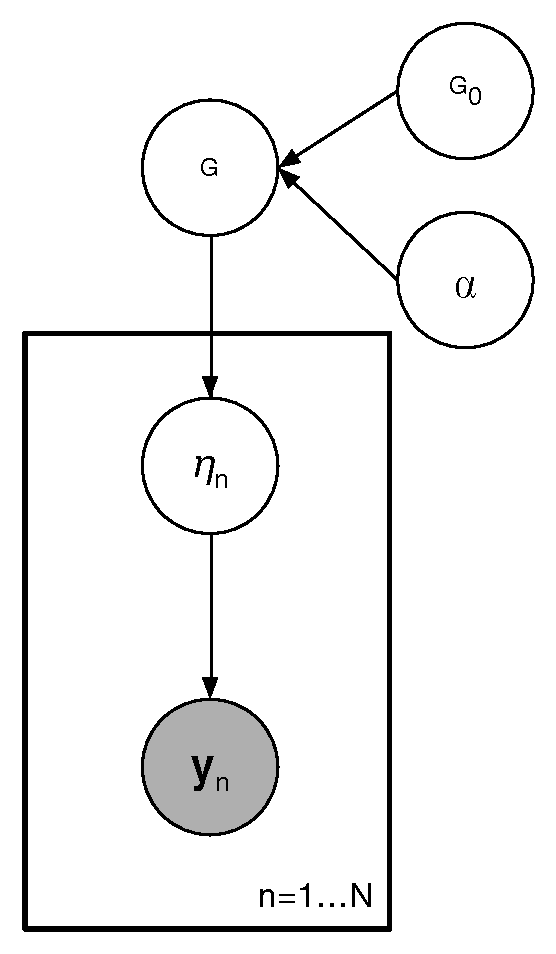
\includegraphics[width=1.5in]{dpmm_pgm}
\caption{PGM for DPMMs}
  \label{fig:dpmm_pgm}
\end{center}
\end{figure}


\subsection{Chinese Restaurant Process Representation}
\begin{itemize}
	\item brief description
	\item generative model
	\item exact inference
		\begin{itemize}
			\item posterior distribution
			\item predictive distribution
		\end{itemize}
	\item Sampling scheme
		\begin{itemize}
			\item Conjugate case
			Gaussian-Gaussian mean /Gamma variance
			Categorical data			
			\begin{itemize}
				\item Non-collapsed
				\item Collapsed
			\end{itemize}
			\item Non-conjugate case
		\end{itemize}
	\item Sampling Algorithm Pseudocode \cite{neal2000markov}
\end{itemize}


\subsection{Stick Breaking Representation}

\begin{itemize}
	\item brief description
	\item hierarchical model
	\item Sampling Algorithm Pseudocode
\end{itemize}

% ----------------------------------------
\section{Experiments}
% ----------------------------------------

\begin{itemize}
	\item One-dimensional data
	\item Higher dimensions
\end{itemize}

\subsection{Synthetic Data}

\subsection{Real Data}

\subsection{Results}
\begin{itemize}
	\item describe clustering accuracy measures used
	\item scatter clustering plot for CRP
	\item scatter clustering plot for SBR
\end{itemize}


% ----------------------------------------
\section{Discussion}
% ----------------------------------------

\subsection{Which one was better?}
\subsection{Future Work}


% ----------------------------------------
% References
% ----------------------------------------

{\footnotesize
\bibliography{ref}
\bibliographystyle{unsrt}
}

% ----------------------------------------
\section{Appendix}
% ----------------------------------------

Sample new cluster assignments as follows:
Question: Do we do steps a, b, c for each iteration (as written below) or do we run the for loop 3 separate times for each step?
\begin{algorithm}
\caption{Rao-Blackwellaized Gibbs Sampler for DPMMs CRP Representation \cite{Sudderth:aa}}
\begin{algorithmic} 
\REQUIRE $z^{t-1} \geq 0 \vee K current cluster statistics$ \\
\STATE (1) $\phi\{1...N\} \sim perm(\{1...N\})$
\STATE (2) $z^{t} \leftarrow z^{t-1} $
\FOR { $ i \in \{\phi(1), \phi(2), ..., \phi(N)\} $ }
\STATE (a)
\FOR {each of the $K$ existing clusters, determine predictive likelihood}
\STATE $f_{k}(x_i) = p(x_i | \{x_j | z_j = k, j \neq i\}, \lambda)$ 
\ENDFOR
\STATE $f_{\bar{k}}(x_i) = p(x_i | z_i = \bar{k}, z_{-i}, x_{-i}, \lambda) = p(x_i | \lambda)$ // reference in the text as how to calculate this
\STATE (b) $z_i \sim \frac{1}{Z_i} (  \alpha f_{\bar{k}}(x_i) \delta(z_i, \bar{k}) + \sum_{k=1}^K N_k^{-i}  f_k(x_i) \delta(z_i, k) ) $ where \\
$ Z_i = \alpha f_{\bar{k}}(x_i) + \sum_{k=1}^K N_k^{-i} f_k(x_i)  $ and $ N_k^{-i} = \# \{x_j : z_j = k\} $
\STATE (c) Update cached sufficient statistics to reflect the assignment of $x_i$ to cluster $z_i$
\IF{$z_i = \bar{k}$ }
\STATE Create a new cluster
\STATE $K \leftarrow K + 1$
\ENDIF 
\ENDFOR 
\STATE (3) set $ z_t \leftarrow z$ // sample mixture parameters current clusters via step 3 of alg 2.1. \cite{Sudderth:aa}
\STATE (4) $K \leftarrow K - \#\{ k : N_k == 0 \} $
\end{algorithmic}
\end{algorithm}

\end{document}